\section{Il Data Warehousing}
Gli strumenti di \textbf{data warehousing} gestiscono la prima trasformazione della BI, dai dati all’informazione. Spesso la troppa disponibilità dei dati, in assenza di uno strumento informatico, rende impossibile l’estrapolazione dell’informazione. 
Una prima definizione di \textbf{Data Warehouse}, ci dice, che è un raccoglitore di informazioni che integra e riorganizza i dati (lo rendo conforme ad un modello) provenienti da sorgenti di varia natura, concentrando tutto dentro al data warehouse e  rendendo di conseguenza i dati disponibile per analisi e valutazioni finalizzate alla pianificazione e al processo decisionale. La cosa che balza all’occhio è che il data warehousing è direttamente consultabile dall’utente finale.

Per capire l’idea alla base delle architetture di data warehousing ci serve creare un distinguo tra due sigle che sono applicate a interrogazioni e più in generale al carico di lavoro, ovvero l’insieme di interrogazioni che più frequentemente gli vengono lanciate sopra:
\begin{itemize}
	\item 
	\textbf{OLTP (On-Line Transactional Processing)}: le query OLTP sono interrogazioni in lettura e scrittura effettuate in tabelle legate da relazioni. La caratteristica di queste query è che nella stragrande maggioranza dei casi sono congelate all’interno dei programmi applicativi. La query SQL non viene creata sul momento dalla logica applicativa, ma questa ha già dei template di query scritte dal programmatore che vengono riempite con i dati dell’utente. Il carico di lavoro è quindi prevedibile, tranne nell’unico caso in cui il DB si è corrotto, e allora in quel caso l’amministratore del DB ha il compito di scrivere una query apposita per risolvere il problema.
	\item 
	\textbf{OLAP (On-Line Analytical Processing}): interrogazioni di natura diversa, ovvero orientati all’analisi. Dal punto di vista strutturale sono diverse da quelle OLTP, intanto perché sono query di sola lettura, e poi perchè mentre  in OLTP il carico è al 99\% congelato, con OLAP si ha un aspetto di interattività molto forte; quindi l’analista decide di volta in volta quali informazioni mostrare. Le nuove query vengono fatte sulle informazioni che vengono mostrate. Quindi il carico di lavoro effettivo varia nel tempo, è prevedibile solo in parte.
\end{itemize}
\begin{figure}[H]
	\centering
	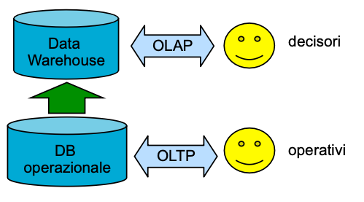
\includegraphics[width=0.7\linewidth]{img/DW}
	\caption{OLAP e OLTP}
	\label{fig:dw}
\end{figure}

Se riprendiamo l’esempio di FIAT, si nota che si ha un problema di prestazioni, perché si è cercato di lanciare una query OLAP sui database relazionali, che non sono progettati e ottimizzati per questo tipo di query. Come si può vedere dalla figura \ref{fig:dw} ho bisogno di separare l’elaborazione di tipo analitico (OLAP) da quella legata alle transazioni (OLTP), costruendo un nuovo repository di dati che è per l’appunto il \textbf{Data Warehouse}. Ho un’architettura con due DB separati: sotto tutti i DB operazionali con gli utenti OLTP che fanno ciò che facevano prima; sopra però creo un nuovo DB, in cui  si integrano tutti i dati che mi arrivano dalla sorgente di sotto, rendendoli disponibili ai decisori per l’analisi OLAP. Ho bisogno che tra i due mondi vi sia qualcuno che permette la sincronizzazione, e ciò è effettuato dall’\textbf{ETL (Extract Transform Load)}, ovvero una procedura batch, non interattiva, lanciata periodicamente per estrarre i nuovi dati che si sono cumulati nell’ultimo intervallo di tempo dalla fonte dei dati. L'ETL ha il compito di pulire i dati, di metterli in una forma diversa e di caricarli nel DW. Da evidenziare come nel DW le informazioni hanno sempre una certa latenza.

Con \textbf{Data Werahousing}, si fa riferimento al processo che estrae i dati e li trasforma in informazione, mentre con \textbf{Data Werahouse}, si fa riferimento al repository.

In particolare, il Data Werahousing è una collezione di metodi, tecnologie e strumenti di ausilio usati per permettere al knowledge worker di fare le sue analisi dei dati finalizzate all’attuazione di processi decisionali e al miglioramento del patrimonio informativo. 

Le \textbf{principali lamentele} sono:
\begin{enumerate}
	\item 
	Abbiamo montagne di dati ma non possiamo accedervi perché non conosco l’SQL per effettuare analisi
	\item 
	Come è possibile che persone che svolgono lo stesso ruolo presentino risultati sostanzialmente diversi?
	\item 
	Vogliamo selezionare, raggruppare e manipolare i dati in ogni modo possibile
	\item 
	Mostratemi solo ciò che è importante
	\item 
	Tutti sanno che alcuni dati non sono corretti
\end{enumerate}

La seconda e l’ultima sono quelle più importanti: spesso interrogazioni uguali forniscono risultati diversi e ancora più frequentemente nel DB sono inseriti dati sbagliati, o peggio ancora non sono proprio stati inseriti.
\subsection{Caratteristiche del processo di Data Warehosuing}
\begin{itemize}
	\item 
	\textbf{Accessibilità}: riferita ad utenti non ICT, non ho bisogno di essere un tecnico informatico, non devo conoscere strutture dati, SQL ecc.
	\item 
	\textbf{Integrazione dei dati}: devo avere una versione unica del dato
	\item 
	\textbf{Flessibilità di interrogazione}: dare all’utente un paradigma di interrogazione che sia non solo accessibile ma anche flessibile, ovvero permettere all’utente di lanciare query complesse mantenendo l’intuitività del programma applicativo
	\item 
	\textbf{Sintesi}: i dettagli inutili vengono scartati ma i dati vengono aggregati
	\item 
	\textbf{Rappresentazione multidimensionale}: le informazioni dentro al DW  vengono caricate in conformità al modello multidimensionale
	\item 
	\textbf{Correttezza e completezza}: pulitura dei dati
\end{itemize}